\subsection{Snižování potřebné náhody}

Nechť běžný (rozhodovací) randomizovaný algoritmus potřebuje $m$ bitů náhody k jedné iteraci a
vydá špatný výsledek s pravděpodobností $p$. Typicky není $p_f$ zrovna dobré a tak
spustíme algoritmus $k$-krát: pokud $k$-odpoví stejně, pravděpodobnost, že se
spletl je $p_f^k$ (typická aplikace je, že se algoritmus plete pouze na jednu
stranu -- tedy pokud jednou odpoví \uv{ne}, nemusíme dál testovat; pokud odpoví
\uv{ano}, mohl se splést). Takový algoritmus potřebuje $k\cdot m$ bitů náhody, což může být problém,
protože počítače jsou stavěné tak, aby byly deterministické, a pravá náhoda se
hledá těžko.

Můžeme si alternativně sehnat expandér (existují deterministické konstrukce),
který má $2^m$ vrcholů, a každému jeho vrcholu přiřadit unikátní $m$-bitové
číslo, znázorňující náhodné bity pro algoritmus. V prvním kroku použijeme $m$
bitů náhody k tomu, abychom zvolili jeden vrchol (prvních $m$ bitů pro
algoritmus). Pro další $m$-tici bitů prostě přejdeme z posledního navštíveného
vrcholu do nějakého jeho souseda, tedy použijeme dalších $(k -1) \cdot \log d$ bitů, kde $d$
je ale nějaká malá konstanta (kdybychom vytvořili úplný graf, máme $d = 2^m-1$ a
dostáváme se na srovnatelnou úroveň s naivním postupem).

Co se stane se pravděpodobností $p_f$? Nemůžeme očekávat, že by zůstala stejná,
ale doufáme, že zůstane dost veliká. Označme $B_x$ množinu všech $m$-bitových
čísel, které pokud jsou použity jako náhoda pro algoritmus, mají za následek, že
algoritmus odpoví špatně pro vstup $x$. Potom víme, že $|B_x|/2^m < p_f$.
Algoritmus selže pouze tehdy, když všechny vrcholy, které v grafu navštívíme,
patří do $B_x$.Pomocí Markovovských řetězců lze dokázat, že pravděpodobnost, že
se toto stane je nanejvýš:
\begin{align}
	\left({|B_x| \over 2^m} + {\lambda_2(G) \over d}\right)^{k-1}
\end{align}
Aplikujeme/li vytah $|B_x|/2^m < p_f$, máme $(p_f + \lambda_2(G)/d)^{k-1}$, což
je stále exponenciální pokles pravděpodobnosti, že algoritmus selže.

\subsection{Min-Cut}

\alg (Kotrakční Min-Cut) Pro graf $G$ zvolme $l$ a dokud $n > l$, kontrahujme
náhodnou hranu. Paralelní hrany zanecháváme, smyčky odstraňujeme.

Kdykoliv má výsledný graf (říkejme mu $G'$) nějaký řez, je tento řez řezem i v
$G$. Speciálně minimální řez v $G'$ je i řezem v $G$; bohužel naopak to neplatí,
protože pokud kontrahujeme hranu, která je obsažena ve všech minimálních řezech,
zvýšíme si tím velikost minimálního řezu alespoň o $1$.

Graf tedy vydá správný výsledek, pokud jsme nekontrahovali hranu v žádném
minimálním řezu. To se dá spočítat. Zafixujme si nějaký minimální řez $C$ s
velikostí $k$. Každý vrchol má stupeň alespoň $k$, protože jinak by hrany s ním
sousedící byly triviálním řezem. Jaká je pravděpodobnost, že vybereme hranu
řezu v nějaké iteraci algoritmu? $p_e \leq k/m \leq k/(kn/2) = 2(n-i+1)$, kde
$i$ je číslo iterace, ve které se kontrakce provádí. Celková pravděpodobnost, že
nevybereme hranu z $C$ je:
\begin{align}
	p \geq \prod_{i=1}^{n-l} \left( 1 - {2 \over n-i+1}\right) =
	\prod_{i=1}^{n-l}{n-i-1 \over n-i+1}
	= {l \cdot (l-1) \over n \cdot (n-1)}
\end{align}
Pokud zvolíme $l=2$, je výsledný řez jasný -- všechny zbývající hrany.
Pravděpodobnost, že ale takto získáme řez minimální, není zrovna dobrá.

\alg (Karger-Stein) Pokud $n < 7$, najdeme řez hrubou silou. Jinak zvolme $l :=
\lceil n/\sqrt 2 +1\rceil$ a spusťme kontrakční algoritmus, a to hned dvakrát, a
zarekurzeme se na oba zkontrahované grafy. Jako výsledek vydej menší z řezů,
které vyšly z rekurze.

Algoritmus zřejmě není horší, než triviální, ale běží o něco rychleji.
Podrobnosti ve skriptíčkách od
MJ\footnote{\url{http://mj.ucw.cz/vyuka/ga/12-randcut.pdf}}.

\subsection{Quick Sort}

\alg Pro vstupní posloupnost prvků $e_i$ zvol náhodně jeden z nich, zarekurzi se
na všechny prvky menší, větší a výsledek zkonkatenuj (zvolený prvek vlož mezi
výsledné dvě posloupnosti.

\vt Střední hodnota počtu porovnání v QuickSortu je $2n \log n$.

\dk Použijeme metodu indikátorů. Všimneme si, že dva prvky $i$ a $j$ (očíslované
od nejmenšího) porovnáme právě tehdy, když je jeden z nich zvolen jako pivot (a
to nanejvýš jednou, protože pivot se již dalšího porovnávání nezúčastní). Nechť
$I_{i,j}$ je indikátor nabývající $1$ pokud k porovnání došlo, $0$ pokud
nikoliv. Zřejmě tedy počet porovnání je $X := \sum_{i < j} I_{i,j}$.

Abychom spočítali střední hodnotu, je potřeba znát pravděpodobnost, že $I_{i,j}
= 1$. K určení hodnoty $I_{i,j}$ dojde právě na jedné hladině -- buď bude jeden
z prvků zvolen jako pivot ($1$), nebo budou rozděleny nějakým jiným prvkem.
Volby pivota, které padnou nalevo od $i$ a napravo od $j$ se $I_{i,j}$ netýkají.
Možností, které zvolí $I_{i,j}$ je tedy celkem ${j-i+1}$ a dvě z toho nastaví
$I_{i,j} := 1$. Máme tedy $P(I_{i,j} = 1) = {2 \over j-i+1}$ a celkem:
\begin{align}
	\sum_{i < j} {2 \over j-i+1} = 2 \cdot \sum_{i=1}^n \left( {1 \over 2} + {1
		\over 3} +
	\dots {1 \over n-i+1}\right)
\end{align}
Kde ale řada v závorce je harmonická řada, která se sečte na $\log n$ a věta je
dokázána. \qed

\subsection{Pravděpodobnostní hierarchie}

Hierarchii vybudujeme pro rozhodovací problémy s jednostrannou chybou, a to
konkrétně pokud na zadání je odpověď {\bf ANO}, algoritmus se může splést a
odpovědět {\bf NE}. Pokud je odpověď {\bf NE}, splést se nemůže a musí vždy
odpovědět {\bf NE}.

\df (RP, co-RP a ZPP) Třída RP je třída algoritmů pracujících v polynomiálním
čase, kde se algoritmus může splést s pravděpodobností nanejvýš $1/2$. Třída
$co$-RP je definovaná se znegovanými odpověďmi (tedy plést se může ${\bf NE}$).
Třída ZPP je průnik obou tříd, tedy algoritmy, které lze řešit
pravděpodobnostně bez chyby, ale čas je omezen pouze ve střední hodnotě.

\poz ZPP lze alternativně definovat jako polynomiálně běžící algoritmus, který
odpoví {\bf ANO}, {\bf NE}, nebo {\bf NEVÍM} s tím, že {\bf NEVÍM} odpoví s
pravděpodobností nanejvýš $1/2$.

\df (BPP) Třída BPP je třída algoritmů pracujících v polynomiálním čase, kde se
algoritmus může splést na obě strany, na každou s pravděpodobností nanejvýš
$1/3$

\df (BQP) Třída BQP jsou pravděpodobnostní algoritmy na kvantových počítačích, a
nemyslím si, že se to někde bralo. Definici neuvádím, zajímavé ale je, že se
očekává, že obsahuje P, obsahuje problémy, které nejsou v NP, ale neobsahuje
celé NP.

\df (PP) Třída PP je třída algoritmů pracujících v polynomiálním čase, kde
algoritmus se může splést na obě strany, na každou s pravděpodobností ostře
méně, než $1/2$.

\poz Třídy BPP a PP vypadají stejně. Rozdíl je ale markantní: u BPP můžeme
spustit algoritmus $k$-krát, podívat se, kolikrát bylo odpovězeno ANO a NE, a
podle toho vydat odpověď (a odhadnout správnost pomocí Černovovy nerovnosti). U
PP to nejde: představme si algoritmus, který pro vstup délky $n$ odpoví špatné s
pravděpodobností $1/2-1/2^n$. To nám trik sice nezakazuje, ale počet opakování,
které musíme získat, abychom se dostali pod nějakou konstantní chybu, je
exponenciální k velikosti vstupu.

\begin{figure}
	\centering
	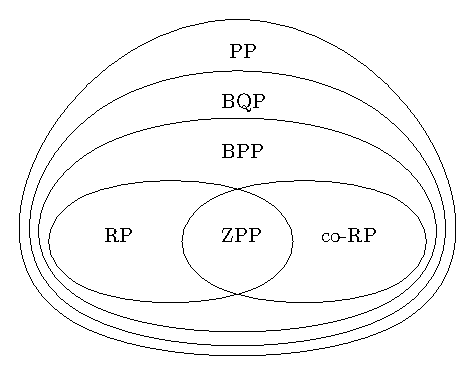
\includegraphics{img/rp-hierarchy.eps}
	\caption{Hierarchie pravděpodobnostních tříd}
\end{figure}

\vt P $\subseteq$ ZPP $\subseteq$ RP $\subseteq$ NP  $\subseteq$ PP $\subseteq$
PSPACE $\subseteq$ EXPTIME

\vt RP$\subseteq$ BPP$\subseteq$ PP

\vt (NP a BPP) Není známo, v jakém vztahu jsou BPP a NP, ale neočekává se, že by
NP $\subseteq$ BPP.

\tv (P ?= BPP) Je otevřený problém, zda P $=$ BPP. Pokud ano, pak P, RP, co-RP a
ZPP jsou si rovny.

\tv (Zero Polynomial Testing) Algoritmus na testování, zda je polynom ve více
proměnných roven nulovému polynomu, je v co-RP, ale  neví se, zda je v P.

\df (Monte Carlo, Las Vegas) Algoritmus, který běží v polynomiálním čase, ale
může vydat špatný výsledek, je {\bf Monte Carlo}. Algoritmus, který běží v
randomizovaném čase, ale vydá správný výsledek vždy, je {\bf Las Vegas}

\subsection{PCP věta}

\df Složitostní třída $\pcp(r(n), q(n))$ je třída jazyků $L$, pro které existuje
polynomiální algoritmus $A(x, \Pi)$ ($x$ je vstup, $\Pi$ je důkaz) tak:
\begin{itemize}
	\item Použije nanejvýš $\O(r(n))$ bitů náhody.
	\item Použije nanejvýš $\O(q(n))$ bitů důkazu.
	\item Pokud vstup $x \in L$, potom existuje $\Pi$ takový, že algoritmus
		$A(x, \Pi)$ vždy odpoví {\bf ANO}.
	\item Pokud vstup $x \notin L$, potom pro každý důkaz $\Pi$ algoritmus
		odpoví {\bf ANO} s pravděpodobností nanejvýš $1/2$.
\end{itemize}

\poz Jako PCP lze definovat některé známé složitostní třídy:
\begin{itemize}
	\item P = $\pcp(0,0)$
	\item NP = $\pcp(0, n^{\O(1)})$
	\item coRP = $\pcp(n^{\O(1)},0)$
\end{itemize}

\vt Pokud $NP \subseteq PCP(\o(\log n), \o(\log n))$, potom P = NP.

\df (PCP) Třídu $\pcp$ definujeme jako $\pcp(\log(n), 1)$.

\vt (PCP Věta) NP = $\pcp$.

A co z toho plyne? Pokud máme libovolný problém v NP, PCP věta nám dává
polynomiální algoritmus na ověření. O tomto algoritmu víme, že potřebuje
$\O(\log n)$ bitů náhody, a k tomu konstantně mnoho bitů z důkazu (nikde se to
nepíše, ale běžně se uvažuje, že je algoritmus neadaptivní -- ve skutečnosti by
to mělo být jedno).

Této vlastnosti lze využít při konstrukci redukce, která pro instanci $3$-SATu
a nějaké $\epsilon$ vytvoří jiný $3$-SAT (nebo jiný problém, na tom tolik
nesejde), takový, že $1-\epsilon$ aproximace nového problému implikuje
splnitelnost starého problému.

\vt (Gap-introducing redukce) Existuje polynomiální transformace T z $3$-CNF
formule na $3$-CNF formuli a $\epsilon > 0$ takové, že:
\begin{enumerate}
		\item Pokud je $\varphi$ splnitelná, $T(\varphi)$ je splnitelná.
		\item Pokud není $\varphi$ splnitelná, pak nanejvýš $1-\epsilon$
			klauzulí $T(\varphi)$ je splnitelných.
\end{enumerate}

To není jednoduché dokázat. Pokud ale takový problém máme, můžeme začít používat
klasické redukce -- speciálně takové, které zachovávají aproximační faktor
(gap-preserving redukce), nebo dokonce takové, které ho zlepšují. Příkladem
toho, jak na to, nechť je důkaz neaproximovatelnosti kliky. Bylo by jednoduché
dokázat, že klika je neaproximovatelná pro nějaké $\epsilon$, prostou redukcí
$3$-SAT na kliku. Následující tvrzení je ale silnější:

\vt (Klika je neaproximovatelná) Je NP-těžké aproximovat maximální kliku v grafu
pro libovolný konstantní aproximační faktor.

\dk Začneme neaproximovatelností $3$-SATu, nechť tedy máme $T(\varphi)$ s $m$
klauzulemi a
$\epsilon$ pro které není $\varphi$ aproximovatelná. Vytvoříme graf $G$
následujícím způsobem: Pro nějaké $c$ nechť jsou vrcholy dvojice $(r,a)$, kde
$r$ je $c$-tice klauzulí (takových $c$-tic bude $m^c$) a $a$ nějaké ohodnocení
proměnných v $r$. Pro každou $c$-tici tedy máme tolik vrcholů, kolik je možných
jejich ohodnocení. Dále spojme hranou všechny vrcholy, které mají nekompatibilní
ohodnocení. Pokud je formule splnitelná, maximální klika má $m^c$ vrcholů. Pokud
je ale nesplnitelná, velikost maximální kliky je nanejvýš $(1-\epsilon)m)^c$.Pro
$c=1$ získáme neaproximovatelnost pro $\epsilon$, protože aproximovatelnost
kliky alespoň $1-\epsilon$ by znamenala stejnou aproximovatelnost $3$-SATu;
pro libovolné větší (ale konstantní) $c$ máme podobnou variantu, ale pro
$(1-\epsilon)^c$ aproximaci, což klesá k nule a tedy klika není aproximovatelná
pro libovolný konstantní aproximační faktor. \qed

